% Template for ICIP-2019 paper; to be used with:
%          spconf.sty  - ICASSP/ICIP LaTeX style file, and
%          IEEEbib.bst - IEEE bibliography style file.
% --------------------------------------------------------------------------
\documentclass{article}
\usepackage{physics}
\usepackage{spconf,amsmath,graphicx, url}
\usepackage{enumitem, booktabs, multirow}
\usepackage[table,xcdraw]{xcolor}
\usepackage{arydshln}

% \usepackage{caption}
% \captionsetup[table]{justification=centerlast,
%                      labelsep=newline,
%                      font=sf,
%                      textfont=footnotesize}
% \captionsetup[figure]{justification=centerlast,
%                      font=sf,
%                      textfont=footnotesize}

\renewcommand\thetable{\Roman{table}} %Make the table's captions Roman numerals
% \setlength{\parskip}{0.1em}

%\parskip 0.2in %Separation between paragraphs
% Example definitions.
% --------------------
\def\x{{\mathbf x}}
\def\L{{\cal L}}
\def\-{\raisebox{.75pt}{-}}
% \renewcommand\thesubsection{\alph{subsection}} %Change subsection from using arabic to alphabetical numbering
% Title.
% ------
\title{System Design SYDE-675 Assignment 1}
%
% Single address.
% ---------------
\name{Gomez Gonzalez, Juan M.}
% For example:
% ------------
\address{University of Waterloo\\
	Department of Electrical and Computer Engineering\\
	200 University Ave W, Waterloo, ON N2L 3G1, Canada}
%
% Two addresses (uncomment and modify for two-address case).
% ----------------------------------------------------------
% \twoauthors
%   {Gomez Gonzalez, Juan M. \textsuperscript{1}}
% 	{\small \textsuperscript{1} Dept. of Electrical and Computer Engineering, University of Waterloo, CA. \\
% 	\small \textsuperscript{2} Dept. of Mechanics and Ocean Engineering, Hamburg University of Technology, DE.}
%   {}
% 	{}

\begin{document}
%\ninept
%
\maketitle

\begin{abstract}
\ninept
\textbf{
This document answers the first assignment for the System Design course SYDE-675, which was taught during the Winter of 2020 at University of Waterloo. It is based on the solutions found using Python, which can be found accompanying this document.
This assignment covers topics including covariance matrices, Naïve Bayes classification, Principal Component Analysis, and Logistic Regression.
} 
\end{abstract}
%
\begin{keywords}
\ninept
Covariance matrix, Principal Component Analysis (PCA), Naïve Bayes, Logistic Regression.
\end{keywords} 
%
% \section{Introduction}
% \label{sec:intro}

\section{Question 1: Data generation based on covariance matrices}
\subsection{Question a: Data samples generation}
\label{subsec:Q1A}
For this question, it was necessary to generate 1000 data samples based on the covariance matrices ($\Sigma$) previously described in the assignment sheet, which can also be seen in Eq. \ref{eq:Q1A_Covs}.

\begin{gather}\label{eq:Q1A_Covs}
% \ninept
\Sigma_A = \begin{bmatrix}
1 & 0\\
0 & 1
\end{bmatrix}
\qquad
\Sigma_B = \begin{bmatrix}
2 & \-2\\
\-2 & 3
\end{bmatrix}
\end{gather}

This means that two groups of samples needed to be sampled from a normal distribution, and afterwards they needed to be modified using the Cholesky decomposition matrix ($L$) by using the previously defined covariance, while also and assuming a mean $\mu$ of zero for the datapoints to be created. This process can be reflected in Eq. \ref{eq:cholesky}

\begin{gather}\label{eq:cholesky}
% \ninept
Samples = L\cdot\Sigma + \mu
\end{gather}

When plotted, this results in two arguably different plots which can be seen in Fig. \ref{fig:Q1A_plot}. This variation in their plots stems from the disparity in their covariances.

% \begin{figure}[!bh]
%     \begin{minipage}[b]{0.48\linewidth}
%       \centering
%       \centerline{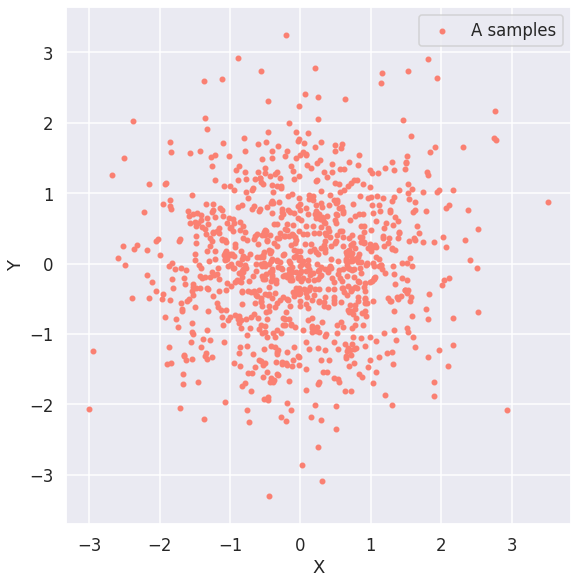
\includegraphics[height = 4.5cm]{Img/Q1A_A.png}}
%       \centerline{(a) A $\Sigma$ Matrix}\medskip
%     \end{minipage}
%     \hfill
%     \begin{minipage}[b]{0.48\linewidth}
%       \centering
%       \centerline{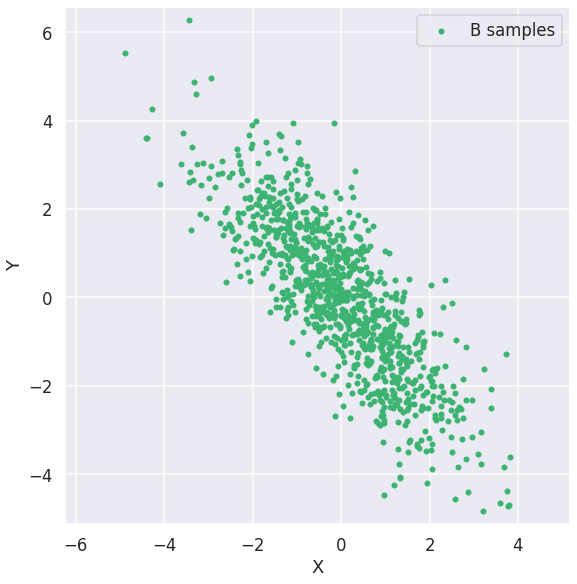
\includegraphics[height = 4.5cm]{Img/Q1A_B.png}}
%       \centerline{(b) B $\Sigma$ Matrix}\medskip
%     \end{minipage}
%     \caption{Scatterplots for A and B $\Sigma$ matrices}
%     \label{fig:Q1A_plot}
% \end{figure}

\begin{figure}[tb]
    \centering
    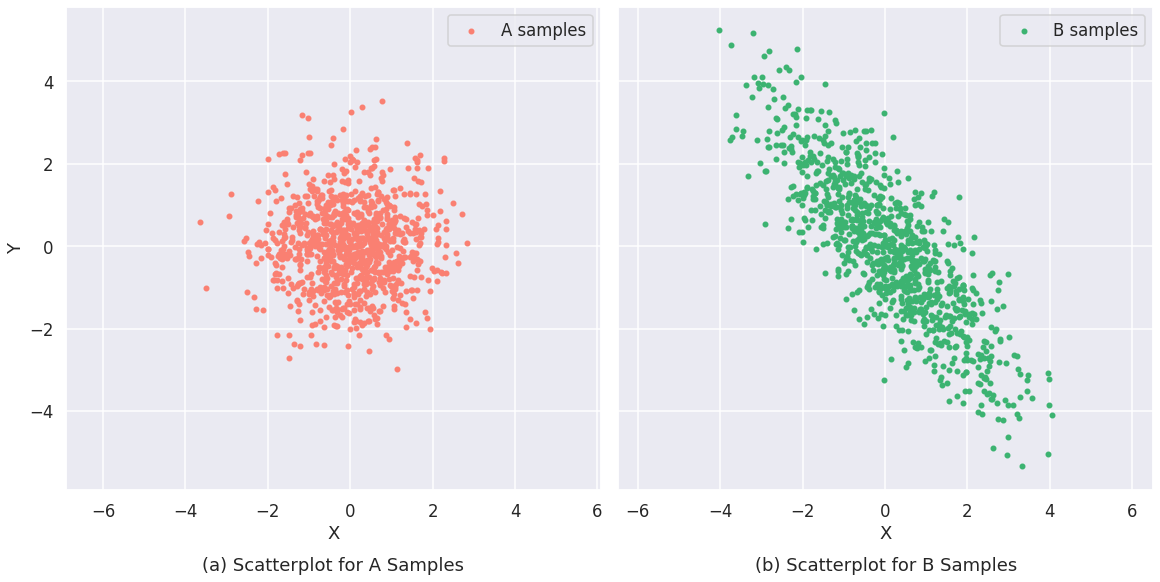
\includegraphics[width=\linewidth]{Img/Q1A.png}
    \caption{Scatterplots for A and B $\Sigma$ samples.}
    \label{fig:Q1A_plot}
\end{figure}

The plots clearly show that Fig. \ref{fig:Q1A_plot} (a) displays equal and uncorrelated variances, making it have a more circular shape compared with Fig. \ref{fig:Q1A_plot} (b), which in turn has a negatively correlated covariance matrix and thus has a more elliptical and tilted data distribution \cite{nazemi_2020}.

\subsection{Question b: Standard deviation contour calculation and plot}
\label{subsec:Q1B}
This question involved calculating the standard deviation contour based on the mean, eigenvalues and eigenvectors of the samples. The samples generated on \ref{subsec:Q1A} were used in solving this problem. First, a function was built in Python in order to find the covariance of a matrix. The covariance can be obtained by substracting the mean  of each feature ($\Bar{x}$ and $\Bar{y}$) to each sample of the dataset ($x_i$ and $y_i$) and then applying the dot product to the transpose of the matrix and the matrix itself. Afterwards, the result of the dot product is divided by the number of samples - 1 ($N - 1$) to finally obtain the covariance matrix\cite{Cov_Calculation}. This process can be seen reflected in Eq. \ref{eq:Q1B}.

\begin{gather}\label{eq:Q1B}
% \ninept
Cov (X,Y) = \tfrac{1}{N - 1} \sum_{i=1}^{n}(x_i - \Bar{x})(y_i - \Bar{y}) = \tfrac{1}{N - 1} \boldsymbol{X^T}\boldsymbol{Y}
\end{gather}

Afterwards, a function to calculate and plot contours was also created. What it would do is use the previously created covariance calculation function to obtain the covariance of the samples, and afterwards would obtain the eigenvalues and eigenvectors using Numpy's Linear Algebra eigh function \cite{Numpy_LinAlg_Eigh}. The square root of the first and second eigenvalues would then be used to calculate the width and height of the ellipse, respectively. The width and height would also be multiplied by the number of standard deviations that are desired to be included in the calculation. This means that for the first standard deviation, which would include approximately 68\% of the datasamples, a value of 1 is needed.

After calculating the width and height, the angle also needs to be calculated so that the ellipse can be rotated according to the data. This can be achieved by obtaining the angle formed by the x axis and the eigenvector corresponding to the largest eigenvalue, which can be obtained by dividing the $Y$ component of the vector by the $X$ component of the eigenvector and applying the inverse tangent function. Fig. \ref{fig:Q1B_plot} shows the previously calculated scatterplots with the resulting contour, using a standard deviation of one.

\begin{figure}[tb]
    \centering
    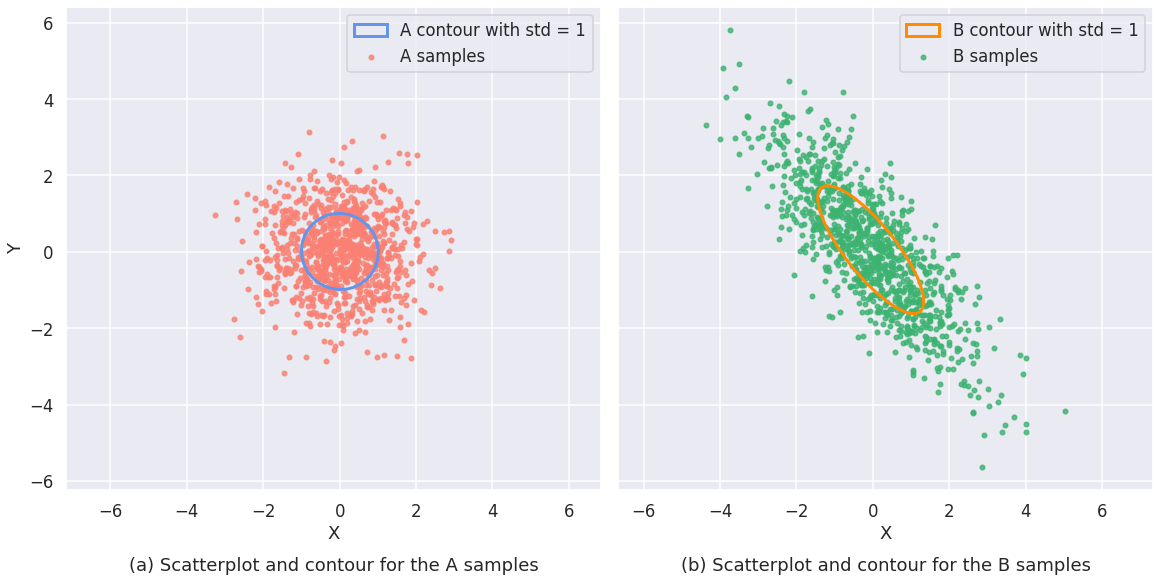
\includegraphics[width=\linewidth]{Img/Q1B.png}
    \caption{Scatterplots and contours for A and B $\Sigma$ samples.}
    \label{fig:Q1B_plot}
\end{figure}

It can be seen in Fig. \ref{fig:Q1B_plot} that the contour follows the shape of the distribution due to it being based on the covariance (which for this case is negatively correlated, as was previously mentioned).

\subsection{Question c: Sample covariance matrices calculation}
\label{subsec:Q1C}
The covariance for the samples can be calculated using the same function created for \ref{subsec:Q1B}. The reuslts can be seen in Eq. \ref{eq:Q1C_Covs}.

\begin{gather}\label{eq:Q1C_Covs}
% \ninept
\Sigma_A = \begin{bmatrix}
1.08 & 0.01\\
0.01 & 1.01
\end{bmatrix}
\qquad
\Sigma_B = \begin{bmatrix}
1.94 & -1.98\\
-1.98 & 2.98
\end{bmatrix}
\end{gather}

Although the results are similar to the covariance matrices from Eq. \ref{eq:Q1A_Covs}, they differ in some decimal places. This discrepancies will be discussed in \ref{subsec:Q1D}.

\subsection{Question d: Difference between sample and "real" covariance matrices}
\label{subsec:Q1D}
Comparing the matrices found in \ref{subsec:Q1C} with the ones defined in Eq. \ref{eq:Q1A_Covs}, it can be seen that although they are similar they are not exactly the same. They both still conserve the property of symmetry and their diagonal is real and positive as well.

Nonetheless, as was previously mentioned, their values differ in some decimals. The reason for their difference is due to the fact that the ones found in \ref{subsec:Q1C} are based on a sample of the whole population, while the ones in \ref{subsec:Q1A} are based on the entire population. They would indeed be equal if the samples were the entire population.

This in turn indicates that the more values we sample from the entire population for our statistical calculations, the more the information obtained from them will approach the real values of the population we are sampling from.

\section{Question 2: MAP and ML Decision Boundaries}
The second question was based on assuming that there were three Classes or groups of samples, described in Eqs. \ref{eq:Q2A_Means}, \ref{eq:Q2A_Covs}, and \ref{eq:Q2A_Probs}.

\begin{gather}\label{eq:Q2A_Means}
\mu_1 = \begin{bmatrix}
3\\
2
\end{bmatrix}
\qquad
\mu_2 = \begin{bmatrix}
5\\
4
\end{bmatrix}
\qquad
\mu_3 = \begin{bmatrix}
2\\
5
\end{bmatrix}
\end{gather}

\begin{gather}\label{eq:Q2A_Covs}
\Sigma_1 = \begin{bmatrix}
1 & \-1\\
\-1 & 2
\end{bmatrix}
\quad
\Sigma_2 = \begin{bmatrix}
1 & \-1\\
\-1 & 2
\end{bmatrix}
\quad
\Sigma_3 = \begin{bmatrix}
0.5 & 0.5\\
0.5 & 3
\end{bmatrix}
\end{gather}

\begin{gather}\label{eq:Q2A_Probs}
P(C_1) = 0.2
\qquad 
P(C_2) = 0.7
\qquad 
P(C_3) = 0.1
\end{gather}

\subsection{Question a: ML and MAP decision boundaries plot}
\label{subsec:Q2A}
For this question, the function created in \ref{subsec:Q1B} for calculating the covariance was used, as well as creating a function that calculates the discriminant using the general case for the Bayes Classifier, which dictates that each class has a different covariance matrix \cite{Bayes_Classifier}. Eq. \ref{eq:Q2A_dsicriminant} shows the expression for this general case.

\begin{gather}\label{eq:Q2A_dsicriminant}
    g_i (x) = X^T W_i x + w_i^T x + w_i0\\
    \notag Where:
    \begin{cases}
      W_i = \tfrac{1}{2} \Sigma^-1\\
      w_i = \Sigma^-1 \mu_i\\
      w_i0 = -\tfrac{1}{2} \mu_i^T \Sigma^-1 \mu_i \- \tfrac{1}{2}  \log(\abs{\Sigma_i}) + \log(P(\omega_i))
    \end{cases}
\end{gather}

For the Maximum A Priori (MAP) case, the probabilities defined in Eq. \ref{eq:Q2A_Probs} were used, while for the Maximum Likelihood (ML) calculation the function assumed equal probabilities for each class (equal to $\tfrac{1}{3}$).

With this discriminant function, the three classes are discriminated and whichever has the highest value is selected as the predicted class for a specific sample. In order to plot the boundaries, a meshgrid\cite{Numpy_Meshgrid} was used and traversed while calculating the discriminant at each coordinate. Afterwards, the contour function created in \ref{subsec:Q1B} was subsequently used to plot each class' ellipse. The mean of each class was also plotted, as requested in the assignment description. Fig. \ref{fig:Q2A_plot} shows the plot with all the requested parameters.

\begin{figure*}[tb]
    \centering
    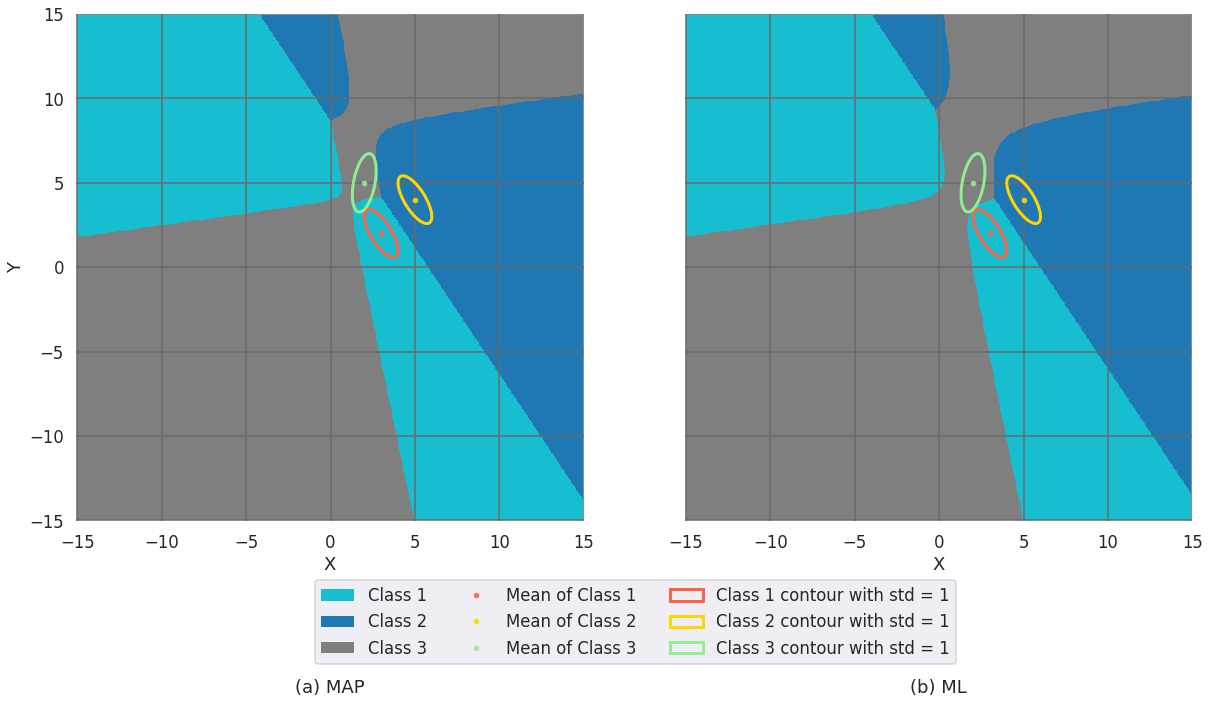
\includegraphics[width=\linewidth]{Img/Q2A.png}
    \caption{Decision boundaries and plot for MAP (a) and ML (b) discriminants}
    \label{fig:Q2A_plot}
\end{figure*}

Comparing both the MAP and ML techniques shown in Fig. \ref{fig:Q2A_plot}, it can be seen that the boundaries are quite similar in general, but diverge in the quadrant between 0 and 5 for both the $X$ and $Y$ coordinates. Looking closely, the decision boundaries for the three classes are different in this area, as Class 1's and Class 2's boundaries are larger for MAP, which makes sense when their probabilities are taken into account. 

To summarize, the previous knowledge of what the probabilities are for each class affect the discriminant function in such a way that it will bias the system to prefer the class with the bigger probabilities over the others.

\subsection{Question b: ML and MAP decision boundaries plot}
\label{subsec:Q2B}
First, 3000 datasamples were selected from a normal distribution. Afterwards, a uniformly random distribution between 0 and 1 was created and sampled from, with one sample of the uniform distribution associated to each sample from the normal distribution. The different classes for the datasamples were then separated based on the value of this uniform distribution, where the samples with a value less than or equal to 0.2 associated to the Class 1, the samples with a value larger than 0.2 and less than or equal to 0.9 associated to Class 2, and the samples with a value larger than 0.9 associated to Class 3.

The 3 classes were then correlated using the Cholesky decomposition in a similar fashion to what was done in \ref{subsec:Q1A}, each Class with its own particular decomposition based on their values reflected in Eqs. \ref{eq:Q2A_Means} and \ref{eq:Q2A_Covs}.

\section{Question 3: PCA}
For this question, the MNIST dataset was used \cite{MNIST_dataset}. It consists of 60,000 samples of handwritten numbers by both american high school students and employees of the United States Census Bureau. Each number is conformed by 28 by 28 pixels in a grayscale image.
\subsection{Question a: PCA Calculation}
\label{subsec:Q3A}
%% One figure
% \begin{figure*}[tb]
%     \centering
%     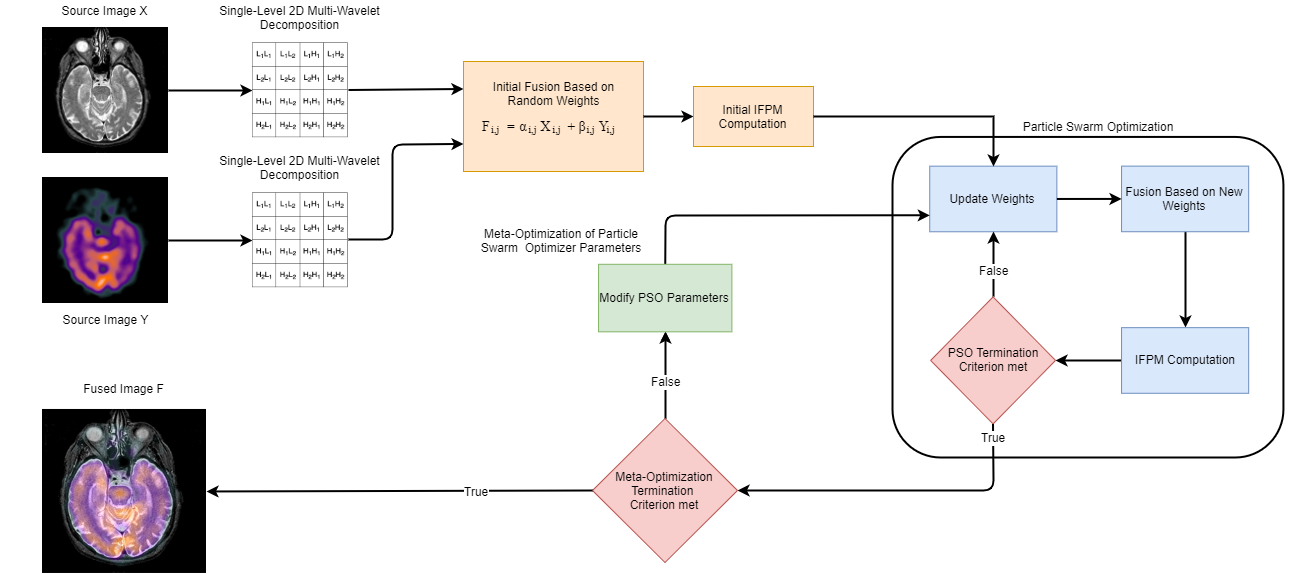
\includegraphics[height=8cm]{Img/Methodology.png}
%     \caption{Flow Chart for the Proposed MRI-SPECT Image Fusion Model. Source images taken from \cite{HarvardBrain}.}
%     \label{framework}
% \end{figure*}
    
% Multiple subfigures in one figure
% \begin{figure}[tb]
%     \begin{minipage}[b]{0.48\linewidth}
%       \centering
%       \centerline{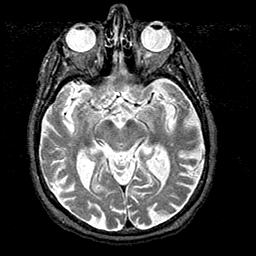
\includegraphics[height = 2.5cm]{Img/S020_MRI.png}}
%       \centerline{(a) MRI Image}\medskip
%     \end{minipage}
%     \hfill
%     \begin{minipage}[b]{0.48\linewidth}
%       \centering
%       \centerline{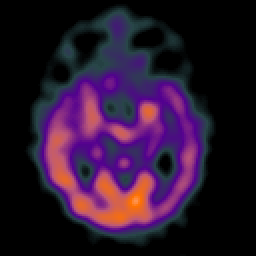
\includegraphics[height = 2.5cm]{Img/S020_SPECT.png}}
%       \centerline{(b) SPECT Image}\medskip
%     \end{minipage}
    
%     \begin{minipage}[b]{0.31\linewidth}
%       \centering
%       \centerline{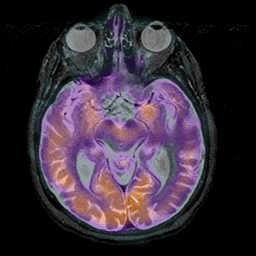
\includegraphics[height = 2.5cm]{Img/S020_Fused_MWT_No_PSO_AVG.png}}
%       \centerline{(c) MWT-AVG}\medskip
%     \end{minipage}
%     \hfill
%     \begin{minipage}[b]{0.31\linewidth}
%       \centering
%       \centerline{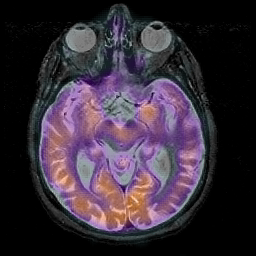
\includegraphics[height = 2.5cm]{Img/S020_Fused_MWT_No_PSO_WANG.png}}
%       \centerline{(d) MWT-WANG}\medskip
%     \end{minipage}
%     \hfill
%     \begin{minipage}[b]{0.31\linewidth}
%       \centering
%       \centerline{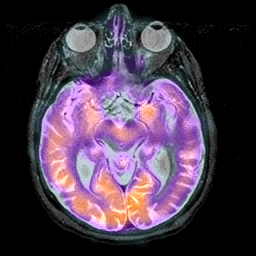
\includegraphics[height = 2.5cm]{Img/S020_Fused_MWT_PSO_Grp.png}}
%       \centerline{(e) MWT-PSO}\medskip
%     \end{minipage}
    
%     \caption{Example of one of the fused images. (a-b) are the MRI and SPECT scans, taken from \cite{HarvardBrain}. Images (c-e) are the fused images obtained using MWT-AVG, MWT-WANG, and MWT-PSO, respectively.}
%     \label{fig:ImgFusion}
% \end{figure}

\section{Conclusion}
\label{sec:conclusion}
% -----------------------b--------------------------------------------------
\bibliographystyle{IEEEbib}
\bibliography{strings,refs}

\end{document}
